\chapter{\texttt{Mesh} class}

\section{Motivation}
To understand, the design behind the Mesh class, we would like to begin by discussing one of the key problems currently faced in \texttt{dgswem}. The issue comes from Steven Brus' dissertation \cite{brusDiss}. Brus goes on to show that the addition of curvilinear elements plays a significant role in obtaining high-order accuracy for real world problems. Simultaneously, these curvilinear elements incur a significantly higher computational cost. Thus in the interior of the finite element domain, where the solution doesn't exhibit mesh geometry to more computationally effient standard affine elements suffice. While computationally straight forward, this approach provides a software engineering challenge. Namely, something like the volume kernel now needs to be split up into two loops, i.e.
\begin{lstlisting}[language=c++, caption={Na\"ive implementation of curved and linear finite element kernel}, label=lst:badloops]
for ( auto& elt : linear_elements ) {
  //Evaluate volume kernel for each linear element
}

for ( auto& elt : curved_elements ) {
  //Evaluate volume kernel for each curved element
}
\end{lstlisting}
This can quickly provide a software engineering headache. For instance, the addition of quadrilateral elements, would suddenly require that each time step cover 4 loops. The addition of more features will lead to more code bloat ultimately resulting in maintainable code. The main goal of the Mesh class is to address specifically the problem, mentioned above.

\section{The Element Class}
The object-oriented solution approach is based on the fact that the discontinuous Galerkin algorithm ultimately, simply applies integrals over the elements, remaining mathematically agnostic to the actually implementation of the approximation. This lends itself to a polymorphic implementation. The idea behind polymorphism being that functionally all elements should behave identically. Thus, if we can agree to an interface that we would like to expose. We should be able to accomplish everything in one loop over the elements without having to worry about what's happening under the hood.

Regardless of the type of element, we assume that for any given element, the approximated solution $u^h$ is given in the form
\begin{equation*}
u^h(x,t) = \sum_{i=0}^{N} u_n(t) \phi_n(x),
\end{equation*}
where $\phi_n$ is some basis. The approximated solution is determined by the evolution of the functions $u_n(t)$. For the Galerkin Method, this evolution is ultimately determined by ensuring that the residuals of the approximate solution is orthogonal to the space spanned by $\{\phi_n\}$. Thus the key functionality that every element must possess is that ability to compute integrals of the form 
\begin{equation*}
\int_{\Omega} f \phi_n \d x
\end{equation*}
for an arbitrary function $f$. In practice these integrations are approximated by quadrature rules. However, this provides the basis for the interface, we would like to expose from a generic element class.
\begin{lstlisting}[language=c++, caption={Generic Element API}]
class Element {

  //Compute the value of F at the Gauss-points
  template <typename F>
  void ComputeFgp(const F& f, std::vector<double>& f_gp);

  //Compute the value of  a function u given by
  // basis coefficients u at the Gauss-Points	    
  void ComputeUgp(const std::vector<double>& u,
                  std::vector<double>& u_gp);

  //Compute the gradient of a function given by
  // basis coefficients u at the Gauss Points    
  void ComputeDUgp(const uint dir,
                   const std::vector<double>& u,
                   std::vector<double>& du_gp);
	
  //Compute the integral of u
  double Integration(const std::vector<double>& u_gp);
	
  //Test u against basis function dof
  double IntegrationPhi(const uint dof,
                        const std::vector<double>& u_gp);
    
  //Test u against the derivative in direction dir
  // of basis function dof
  double IntegrationDPhi(const uint dir,
                         const uint dof,
                         const std::vector<double>& u_gp);

  //...
};
\end{lstlisting}
That is to say if every element satisfied this API, we would be able to write the discontinuous Galerkin kernel with only one loop regardless of the element.

\subsection{Strong Typing}
C++ is a strongly typed language. Thus, in exposing any kind of polymorphism there are two options. (1) Dynamic polymorphism and (2) Static polymorphism. Dynamic polymorphism is typically achieved through the use of the  \lstinline[language=c++]{virtual} keyword. This approach is typically considered the most readable, and typically be preferred in a first attempt at an implementation. However, virtual objects typically can't be resolved by the compiler at runtime. This means that when the executable is running, the compiler maintains a virtual look-up table, which it uses to determine which implementation to call, when provided one of these virtual calls. The cost of this is that there is a virtual overhead associated with each of these calls. Additionally, the compiler may have trouble inlining and optimizing virtual function calls. Typically, when the function execution is large enough this overhead may be treated as negligible. But for our applications, these function calls are expensive enough that virtualization would seriously degrade performance. 

The other typical approach is the use of static polymorphism. The idea being that we still maintain a unified API exposed by the class. However, now we specify the order in which we loop through the elements. That way the compiler is able to determine each of the function calls. Although ultimately, we will be able to get away with still only having one loop. The binary code generated should be equivalent to the code in Listing \ref{lst:badloops}. Thus, static polymorphism provides us with the usage of dynamic polymorphism without the additional overhead. The downsides include a code base that is more difficult to maintain. However, given the performance critical nature of these function calls, this is a downside we've decided to accept.

\subsection{Class Hierachy of Element}
\begin{figure}
\centering
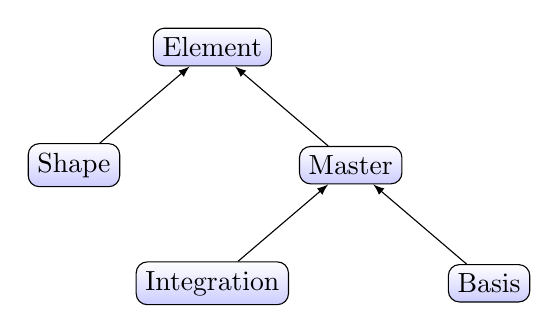
\begin{tikzpicture}[edge from parent/.style={draw,<-,>=latex}, sibling distance=10em,
  every node/.style = {shape=rectangle, rounded corners,
    draw, align=center,
    top color=white, bottom color=blue!20}]]
  \node {Element}
    child { node {Shape} }
    child { node {Master}
      child { node {Integration} }
      child { node {Basis} } };
\end{tikzpicture}
\caption{Composition of the Element classes.}
\label{fig:eltcomp}
\end{figure}
The last subsection describes the exact decomposition of the element. In designing \texttt{dgswem-v2}, we attempted to think of all possible features that one might want to implement and provide encapsulation to allow for adding of new features without having to be familiar with the entire code base. Figure \ref{fig:eltcomp} describes the major constituents of the element class.
\begin{itemize}
\item \textbf{Shape}: The shape class deals with deformations from the master element to the actual orientation within the mesh. Here features such as curvature of the mesh (e.g. solving in spherical coordinates) or the element (e.g. isoparametric or isogeometric) should be implemented.
\item \textbf{Master}: The master element is rather similar to the generic element class. It exposes integration hooks over the master element.
\item \textbf{Basis}: This class encapsulates all basis information. Potentially additional choices of basis include Bernstein, modal, and bases on quadrilateral elements.
\item \textbf{Quadrature}: This class contains all information required to approximate an integral over the master element. 
\end{itemize}
In addition to adding features by providing new instances of these classes. There also still remains the ability to add classes through template specialization and SFINAE. These techniques allow for special implementations to be written in certain element compositions. For example, one of the large advantages of a Bernstein basis is the fast matrix inversion formula. Since this formula drastically deviates from linear elements, one might want to write a specific implementation for linear triangles using the Bernstein basis. 
\section{\texttt{Mesh} Class}
With the decision to strongly type the elements in the Mesh class, the next task is to develop a container, which represents the mesh. This requires the ability to iterate over interfaces, boundaries, elements, and distributed boundaries. The key object in allowing this to are the heterogeneous containers in the \textbf{Utilities} namespace. To explain, what in particular is happening in these containers assume we have three types of elements in our mesh: \lstinline{EltA, EltB, EltC}.
Morally, the heterogeneous vector can be written out as:
\begin{lstlisting}[language=c++]
using HeterogeneousVector<EltA,EltB,EltC> = tuple<vector<EltA>,
                                                  vector<EltB>,
                                                  vector<EltC>>;
\end{lstlisting}
Now assuming, we have a function we would like to execute on each element regardless of type. We emulate the \lstinline[language=c++]{std::for_each} API. So we will define a hook in the Mesh class, which will execute that function for every element in the HeterogeneousVector. We have demonstrated what specifically we would like in Listing \ref{lst:foreach}.
\begin{lstlisting}[language=c++,
                   caption={Moral implementation of iterating over HeterogeneousVector},
                   label=lst:foreach]
template<typename Element>
void SomeKernel(Element& e);                   
                   
template<typename F>
void ForEachImpl( HeterogeneousVector<EltA,EltB,EltC>& v,
                   const F& f ) {

  vector<EltA>& vA = get<0>(v);
  for_each(vA.begin(),vA.end(), f);
  
  vector<EltB>& vB = get<1>(v);
  for_each(vB.begin(), vB.end(), f);
  
  vector<EltC>& vC = get<2>(v);
  for_each(vC.begin(), vC.end(), f);
}

//Apply SomeKernel to every element in v
MoralForImpl(v, SomeKernel);
\end{lstlisting}
In \texttt{dgswem-v2}, this type of implementation can be generalized to arbitrary Hetereogeneous vectors through the use of template metaprogramming. However, ultimately, the code is effectively executing the above code. Allowing the compiler to generate these loops is precisely the issue we wanted to address. The definition of the kernels to be passed into the mesh class are problem specific and will be addressed in the next chapter. This mechanism is used for boundaries, internal interfaces, and distributed interfaces, in addition to elements. In understanding, this key concept the Mesh class becomes nothing more than a container. Detailed API descriptions are provided in the doxygen documentation.